\documentclass[a4paper,14pt]{extarticle}
\usepackage[english,russian]{babel}
\usepackage[cache=false]{minted}
\usepackage{fontspec}
\usepackage{indentfirst}
\usepackage{listings}
\usepackage{color}
\usepackage{caption}
\usepackage{amsmath}
\usepackage{hyperref}
\usepackage{graphicx}
\usepackage[%
    left=20mm,%
    right=10mm,%
    top=20mm,%
    bottom=20mm,%
]{geometry}%
\usepackage{titlesec}


\setmainfont{PT Astra Serif}

\hypersetup{
    colorlinks=true,
    linkcolor=black,
    filecolor=magenta,
    urlcolor=cyan,
    pdftitle={Лабораторная работа №4},
    pdfpagemode=FullScreen,
}

\newcommand{\hlink}[2]{\href{#1}{\color{blue}\underline{#2}}}
\graphicspath{ {./images/} }

\setmonofont[Scale=0.8]{JetBrains Mono}
\setminted{frame=lines, framesep=3mm, fontsize=\small}
\usemintedstyle{vs}

\titleformat{\section}
{\normalfont\bfseries}{}{0pt}{Упражнение \thesection.\;}

\titleformat{\subsection}
{\normalfont\bfseries}{}{0pt}{Задание \thesubsection.\;}

\numberwithin{figure}{section}

\begin{document}

\begin{titlepage}
    \vspace{0pt plus2fill}
    \noindent

    \vspace{0pt plus6fill}
    \begin{center}
        \textbf{\large{Санкт-Петербургский национальный исследовательский университет информационных
                технологий, механики и оптики}}

        \vspace{0pt plus2fill}
        \textbf{\Large{ЛАБОРАТОРНАЯ РАБОТА №8}}

        \vspace{0pt plus2fill}
        \textbf{\large{Использование интерфейсов при \\ реализации иерархии классов}}
    \end{center}

    \vspace{0pt plus8fill}
    \begin{flushright}
        Студент: \\
        \textit{Швалов Даниил Андреевич}

        \textit{Факультет ИКТ}

        Группа: \textit{К32211}

        Преподаватель: \\
        \textit{Иванов Сергей Евгеньевич}
    \end{flushright}

    \vspace{0pt plus4fill}
    \begin{center}
        {Санкт-Петербург~--- 2023}
    \end{center}
\end{titlepage}

\section{Создание и реализация интерфейса}

В проект был добавлен интерфейс \texttt{IPubs}, содержащий метод \texttt{Subs} для проверки подписки и свойство \texttt{IfSubs} для оформления подписки:

\inputminted{csharp}{../MyClass/MyClass/IPubs.cs}

Класс \texttt{Magazine} был унаследован от интерфейса \texttt{IPubs}. Также были реализованы свойства и методы, объявленные в интерфейсе:

\inputminted{csharp}{../MyClass/MyClass/Magazine.cs}

Классы \texttt{Book} и \texttt{Item} остались без изменений:

\inputminted{csharp}{../MyClass/MyClass/Book.cs}

\inputminted{csharp}{../MyClass/MyClass/Item.cs}

В класс \texttt{Program} был добавлен код, проверяющий работу программы:

\inputminted{csharp}{../MyClass/MyClass/Program.cs}

На рис. \ref{fig:task-1} представлен пример работы программы.

\begin{figure}[H]
    \centering
    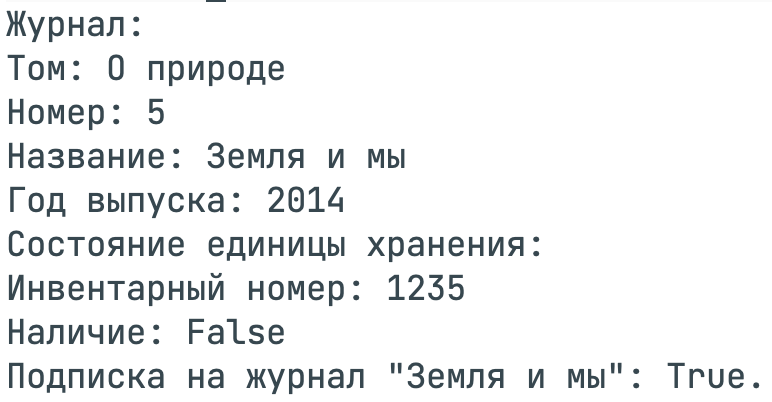
\includegraphics[width=0.5\textwidth]{images/task-1.png}
    \caption{Пример работы программы}
    \label{fig:task-1}
\end{figure}

\section{Использование стандартных интерфейсов}

В класс \texttt{Item} было добавлено наследование интерфейса \texttt{IComparable}, а также был реализован метод этого интерфейса \texttt{CompareTo} по полю \texttt{invNumber}:

\inputminted{csharp}{../MyClass1/MyClass/Item.cs}

Остальные классы остались без изменения:

\inputminted{csharp}{../MyClass1/MyClass/IPubs.cs}

\inputminted{csharp}{../MyClass1/MyClass/Book.cs}

\inputminted{csharp}{../MyClass1/MyClass/Magazine.cs}

В класс \texttt{Program} был добавлен код, проверяющий работу программы:

\inputminted{csharp}{../MyClass1/MyClass/Program.cs}

На рис. \ref{fig:task-2} представлен пример работы программы.

\begin{figure}[H]
    \centering
    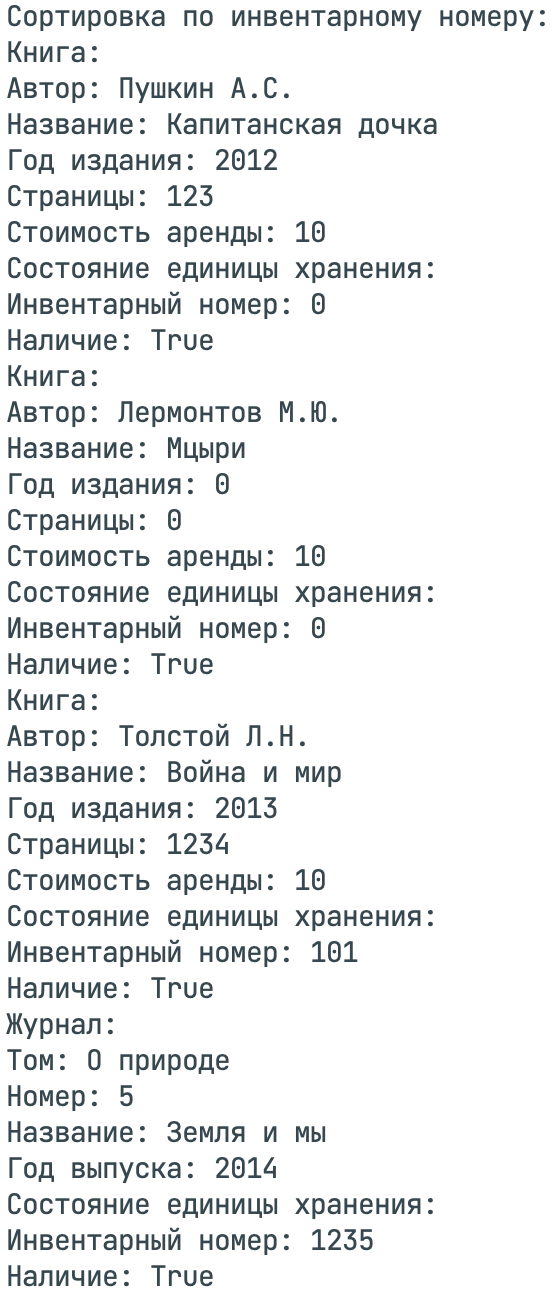
\includegraphics[width=0.5\textwidth]{images/task-2.png}
    \caption{Пример работы программы}
    \label{fig:task-2}
\end{figure}

\section{Реализация прогрессии с помощью интерфейса}

Абстрактный класс \texttt{Progression} был заменен на интерфейс \texttt{IProgression}:

\inputminted{csharp}{../Progression/IProgression.cs}

Классы \texttt{ArithmeticProgression} и \texttt{GeometricProgression} были переделаны под использование этого интерфейса:

\inputminted{csharp}{../Progression/ArithmeticProgression.cs}

\inputminted{csharp}{../Progression/GeometricProgression.cs}

В класс \texttt{Program} был добавлен код, проверяющий работу программы:

\inputminted{csharp}{../Progression/Program.cs}

На рис. \ref{fig:task-3} представлен пример работы программы.

\begin{figure}[H]
    \centering
    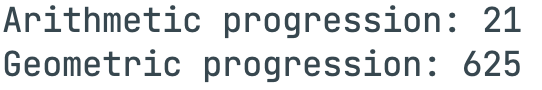
\includegraphics[width=0.5\textwidth]{images/task-3.png}
    \caption{Пример работы программы}
    \label{fig:task-3}
\end{figure}

\end{document}
